\part{File System}

\chapter{General Principles}

\section{About vnodes and inodes}

During this document terms \acs{vnode} and \acs{inode} are unfortunately used
interchangeably. Historically inode was the way to index files in Unix-style
file systems.\cite{Wikipedia:inode} While Zeke continues this fashion it adds
a concept of vnodes that are used as an abstraction level between actual file
systems and \acf{vfs}. This concept is not new by any means but reader has to
be familiar with the concept especially due to the mixed terminology in this
document.

To sum up, vnodes are used from user level to \acs{vfs} level and actual file
system implementations are using internally inodes and externally vnodes.

\section{Kernel Interface}

Kernel interface to ramfs is built around virtual function structs defined in
\acs{vfs} header file \verb+fs.h+ and some user space header files defining
unified data types.

A new file system is first registered to the kernel by passing a pointer to
fs struct that is an interface to mount a new superblock, ramfs in this case.
This struct is defined as in listing \ref{list:fs}.

When superblock is mounted a superblock struct pointer is returned. This pointer
servers as the main interface to the newly mounted file system. Superblock is
defined as in listing \ref{list:fs_sb}. By using superblock function calls it's
possible to get direct references to vnodes and \acs{vnode} operations e.g. for
modifying file contents or adding new hard links to a directory node.

\lstinputlisting[label=list:fs,caption=fs struct definition.]{fs/fs.c}
\lstinputlisting[label=list:fs_sb,caption=superblock struct definition.]{fs/fs_superblock.c}

Currently supported vnode operations are listed in listing \ref{list:vnode_ops}.
Names of these operations are selected to somewhat match with the corresponding
function names defined in \acs{POSIX}. Albeit arguments of the \acs{vfs} level
functions are quite different from the user level.

\lstinputlisting[label=list:vnode_ops,caption=Supported vnode operations.]{fs/vnode_ops.c}

\chapter{ramfs}
\section{Overall description}

The purpose of the \acs{ramfs} is to provide a storage in RAM for temporary
files. This is important in user scope where there might be no other writable
storage medium available on some embedded platform. In addition to storage
for temporary files in user scope ramfs could be useful to store kernel files
as well, e.g. init can be unpacked from kernel to ramfs and then executed.

In the future ramfs code might be also useful for \acs{vfs} caching, so that
changes to a slow medium could be stored in ramfs-like structure and synced
later.

Ramfs should implement the same \acs{vfs} interface as any other regular
file system for Zeke. This ensures that the same POSIX compliant file
descriptor interface\footnote{POSIX file API is not actually yet implemented.}
can be used for files stored to ramfs as well as to any other file system.

\section{Structure of ramfs}

Data in Ramfs is organized by inodes, \acs{inode} can contain either a file or
directory entries, which means that an inode can be either files or directories.
Maximum size of a mounted ramfs is limited by size of \verb+size_t+ type.
Maximum size of a file is limited by size of \verb+off_t+ type. Figure
\ref{figure:inodes} shows a high level representation of how inodes are
organized and linked in ramfs to form directory tree with files and directories.

Contents of a file is stored in blocks of memory that are dynamically allocated
on demand. Block size is selected per file so all blocks are equal size and
block pointer array (\verb+in.data+) is expanded when new blocks are allocated
for a file. Figure \ref{figure:file} shows how memory is allocated for a file
inode.

Directory in ramfs is stored similarly to a file but \verb+in.dir+ (union with
\verb+in.data+) is now constant in size and it's used as a hash table which
points to chains of directory entries (directory entry arrays). If two files are
mapped to a same chain by hash function then the corresponding chain array is
re-sized so that the new entry can be added at the end of array. This means that
lookup from a directory entry chain is quite cache friendly and can usually
avoid fragmentation in memory allocation. Figure \ref{figure:dir} represents a
directory inode containing some directory entries.

\begin{figure}
  \center
  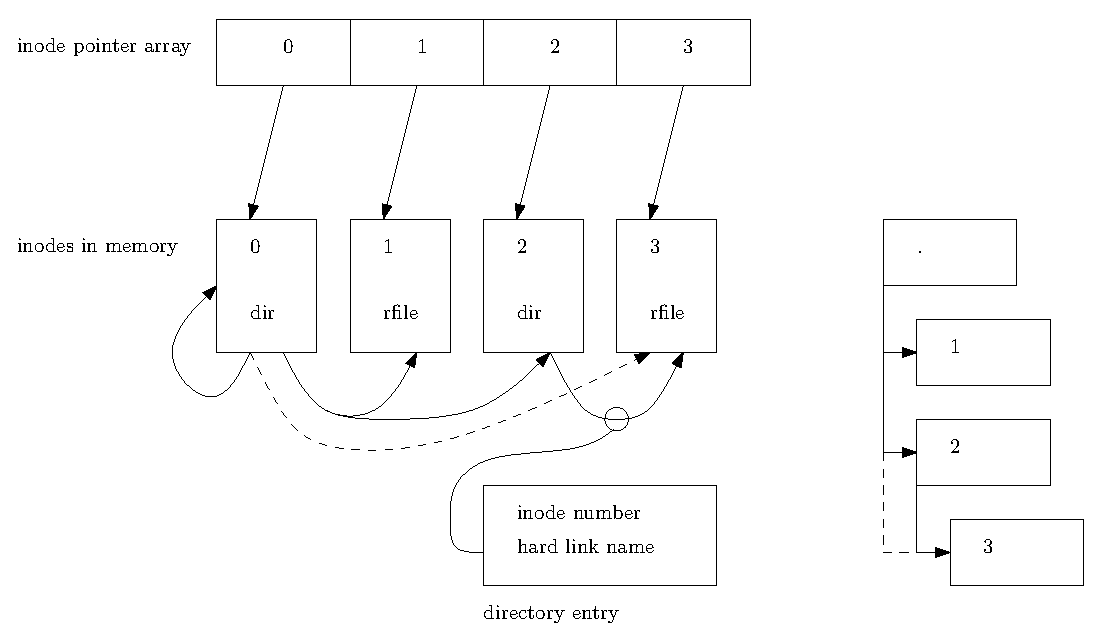
\includegraphics[width=15cm]{pics/inodes}
  \caption{Mounted ramfs with some inodes.}
  \label{figure:inodes}
\end{figure}

\begin{figure}
  \center
  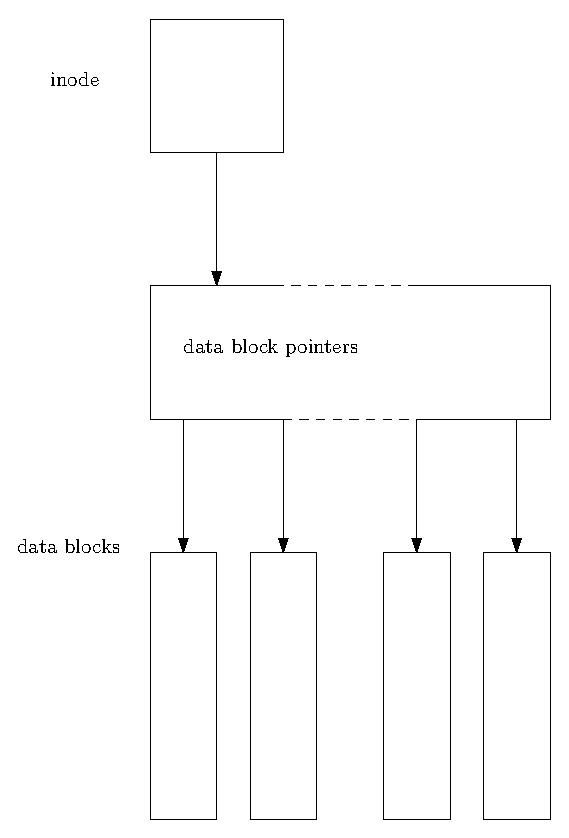
\includegraphics[width=7cm]{pics/file}
  \caption{Structure of a file stored in ramfs.}
  \label{figure:file}
\end{figure}

\begin{figure}
  \center
  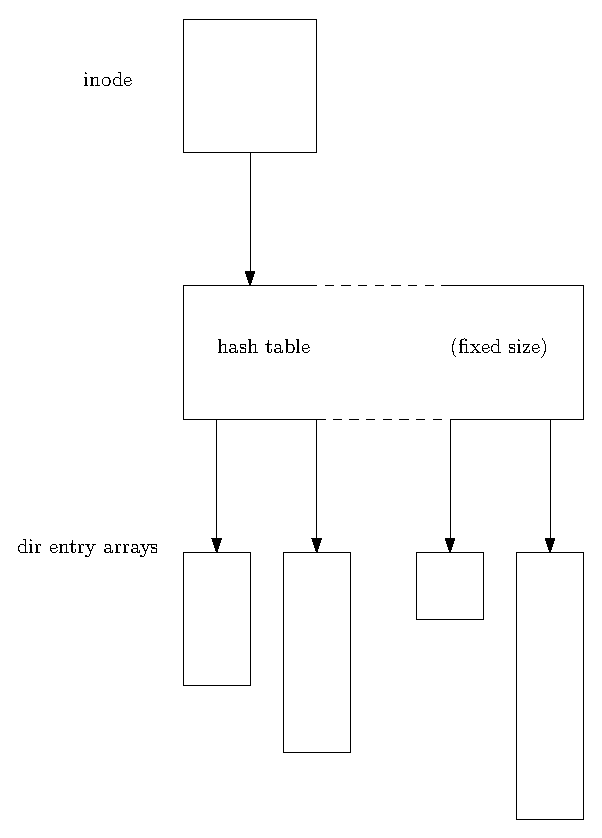
\includegraphics[width=7cm]{pics/dir}
  \caption{Directory containing some directory entries in ramfs.}
  \label{figure:dir}
\end{figure}


\section{Time Complexity and Performance Analysis}

\subsection{Mount}

When a new ramfs superblock is mounted it's appended to the end of the global
superblock list. Time complexity of this operation is $O(n)$ as there is no
information about the last node in the list. However this is not a major
problem because new mounts happen relatively rarely and other operations during
the mounting process will take much more time than traversing a super block list
of any practical length. Those other operations includes allocating memory for
inode array, allocating memory for inode pool and initializing some data
structures etc.

\subsection{Get vnode by vnode number}

Index nodes are stored in contiguous array as shown in figure
\ref{figure:inodes}. This trivially means that a vnode can be always fetched
from mounted ramfs in $O(1)$ time as it's only a matter of array indexing.

\subsection{Lookup vnode by filename}

File lookup on ramfs level is implemented only on single directory vnode level
and sub-directory lookup must be then implemented on \acs{vfs} level i.e. lookup
function for a vnode can only lookup for entries in the current directory
vnode. A file lookup is made by calling \verb+vnode->vnode_ops->lookup()+.    

Directory entries are stored in chained hash tables as shown in figure
\ref{figure:dir}. It can be easily seen that usually a chain array contains only
a single entry and therefore lookup is $O(1)$. In sense a of performance and
efficiency of a chain array with length greater than zero is more complex.
Trivially lookup from array is of course $O(n)$. What is interesting here is
how CPU caching works here. Even though directory entries are different in size
they are all stored in contiguous memory area and can be loaded to CPU cache
very efficiently, whereas many other data structures may lead to several
non-contiguous memory allocations that will pollute the caching and slow down
the lookup if there is only few entries. That said the current implementation of
directory entry storage seems almost perfect solution if amount of directory
entries is moderate and hash functions is good enough.\cite{Wikipedia:htable}

\subsection{Data by vnode}

Data stored in file inodes is accessed by calling
\verb+vnode->vnode_ops->read()+ and \verb+vnode->vnode_ops->write()+. Arguments
for both contains a pointer to the vnode, offset where to start reading or
writing from, byte count and a pointer to a buffer. Data structuring of a file
vnode was illustrated in figure \ref{figure:file}.

Pointer to a block of data by \verb+offset+ is calculated as shown in equation
\ref{eqn:dpointer}, where data is the data block pointer array. Length of
data pointer by the pointer is calculated as shown in equation \ref{eqn:dlen}.

\begin{eqnarray}
  \textrm{block} &=& \textrm{data} \left[ \frac{\textrm{offset} -
    (\textrm{offset} \& (\textrm{blksize} - 1))}{\textrm{blksize}}
    \right] \\
  \textrm{p}     &=& \textrm{block} \left[ \textrm{offset} \& (\textrm{blksize} - 1)
    \right] \label{eqn:dpointer} \\
  \textrm{len}  &=& \textrm{blocksize} - (\textrm{offset} \& (\textrm{blksize} - 1)) \label{eqn:dlen}
\end{eqnarray}

\subsection{Create a vnode}

Normally when a new inode is created it can be taken from the inode pool and
inserted at empty location on inode array. Average case can be considered to be
$O(1)$ then.

Lets consider a case where a new vnode is created and inserted to the index node
array but it's already full. A call to \verb+krealloc()+ will be issued and the
worst case of reallocation of a memory location may require to create a copy
of the whole index node array to a new location. This means that the worst case
time complexity of a vnode creation is relative to size of the array, so its
$O(n)$.

\subsection{Summary}

\begin{table}
  \caption{Summary of time complexity of ramfs functions.}
  \label{table:complexity}
  \begin{tabular}{lcc}
    Function & Average time complexity & Worst case time complexity \\
    \hline
    mount                 & $O(n)$ & $O(n)$ \\
    vnode by vnode number & $O(1)$ & $O(1)$ \\
    vnode by filename     & $O(1)$ & $O(n)$ \\
    data by vnode         & $O(1)$ & $O(1)$ \\
    create a new vnode    & $O(1)$ & $O(n)$
  \end{tabular}
\end{table}


\section{Performance Testing}

Automated performance tests were implemented the same way as unit tests.
Ramfs performance tests are in \verb+test_ramfsperf.c+ file.

\subsection{Test Results}

\subsection{Hard link operations}

Performance of hard link operations is tested in \verb+test_dehtableperf.c+.

Figure \ref{figure:dhlink_perf} shows performance measurements from
\verb+test_link_perf()+ test. In this test number of randomly named nodes are
added at every point and total time of adding those links is measured.
Name collisions are not handled but just appended to the chain array.
It seems that total time of \verb+dh_link()+ calls is almost flat but
it then starts to smoothly transform to something that is almost linearly
relative to the amount of links added. Calls to \verb+kmalloc()+ and
\verb+krealloc()+ seems to add some random behavior to link times.

Lookup tests were performed with \verb+test_lookup_perf()+ test and illustrated
in figure \ref{figure:dhlookup_perf}. The test works by first adding certain
amount of randomly named links and then trying to lookup with another set of
randomly selected names. Hit percentage is named as "\% found" in the plot and
lookup time is the mean of 100 random lookups. Lookup function seems to behave
quite linearly even though there is some quite strange deviation at some link
counts.

Even though lookups seems to be in almost linear relationship with the link
count of the directory entry hash table it doesn't mean lookups are slow.
Even with 20000 links average lookup takes only $45\:\mu s$ and it's very
rare to have that many directory entries in one directory.

\begin{figure}
  \includegraphics[width=15cm]{plots/dh_link}
  \centering
  \caption{Directory entry hash table link performance.}
  \label{figure:dhlink_perf}
\end{figure}

\begin{figure}
  \includegraphics[width=15cm]{plots/dh_lookup}
  \centering
  \caption{Directory entry hash table lookup performance.}
  \label{figure:dhlookup_perf}
\end{figure}

\subsubsection{File operations}

Performance tests for file operations were performed on the universal target
where kmalloc uses malloc instead of dynem block allocator, this in fact may
make some of the result unreliable.

\begin{tabular}{l r@{.}l}
\textbf{Operation} &
\multicolumn{2}{c}{\textbf{Transfer speed (MB/s)}} \\
\hline
\textbf{Single write (100 MB)} && \\
new file      & 21&62 \\
existing file & 1694&92 \\
read          & 1098&90 \\
\textbf{Sequential writes} && \\
new file      & 9&06 \\
existing file & 335&80 \\
read          & 426&22 \\
\end{tabular}

\subsubsection{ramfs write/read performance}

Write and read performance testing is somewhat biased by the underlying kernel
even though we have our own memory allocator in place. Actually kmalloc may
make things work even worse because it's optimized for different kind of
suballocator that is not present on API level of Linux. So I think this is a
major cause for very poor memory allocation and first pass write performance
to the allocated blocks of memory, although kmalloc it self is quite inefficient
too.


\section{Suggestions for Further Development}

\subsubsection{Directories}

Directory entry lookup tables (hash tables) could be made variable in size.
This would make use of directory entry chains less frequent and greatly improve
performance of large directories while still maintaining small footprint for
small directories containing only few entries. At minimum this would only
require a function pointer to the current hash function in the inode. There is
no need to store the size of current hash table array in variable because it can
be determined by comparing the function pointer. So overhead of this improvement
would be size of \verb+size_t+ per directory and one more dereference per lookup.


\chapter{devfs}
\section{Introduction}

Devfs inherits ramfs and creates an abstraction layer between device drivers
and device driver abstraction layers. Essentially devfs creates a file
abstraction with vfs read() and write() functions that communicates with the
actual device driver.

\section{Device creation process}

Device registration with devfs starts from static init function of a subsystem,
device detection routine or some other triggering method. The device
identification/creation function shall, by some way, create a \verb+dev_info+
struct that describes the device and provides necessary function pointers for
reading and writing. Then \verb+make_dev(devXXX_info, 0, 0, 0666)+ is called
to register the device created. \verb+make_dev()+ then creates a fs node that is
contains a pointer to the provided \verb+dev_info+ in \verb+vn_specinfo+ of the
device.

There is some notable differences between devfs implementation of Zeke and other
common devfs or device abstractions in some other operating systems,
particularly Unices. First of all we don't use majorminor combination as a
device idetentifier, it's only provided for compatibility reasons and not used
for anything actually.\footnote{Some drivers may still use those internally but
there is no external interface provided. Uart is one of those using minor
numbers for internal indexing.} So devices can't be accessed by creating
a device file anywhere in the system, device files in Zeke are very special and
only ones that are created with \verb+make_dev()+ are valid, since the object
oriented model of Zeke VFS.

Another difference is that Zeke does not have character and block device
access modes/file types like most of traditional Unices. Zeke can support
buffered writes but it's always hidden from the user space. In practice,
it means that every user reading from a device file will always see the
same state, eg. if one process would write by using block device and another
one reading character device, the latter one would get either old data or
corrputed data. In fact there is no reason to have different file types for
different device types, block device files were designed to be a special file
type for hard disks, for some reason, but it doesn't make any sense to do it
that way in a modern kernel.\cite{Kamp:rethinkdev} Thus block device files are
not supported in Zeke and buffered access is not implemented but technically
supported inside the kernel.

\section{UART devices}

UART devices are handled by UART submodule (\verb+kern/hal/uart.c+) so that
common code between UART implementations can be shared and tty numbering can
be centrally organized. To register a new UART port the device driver has to
allocate a new \verb+uart_port+ structure and pass it to
\verb+uart_register_port()+ which finally registers the a new device file for
the port.

\begin{figure}
  \center
  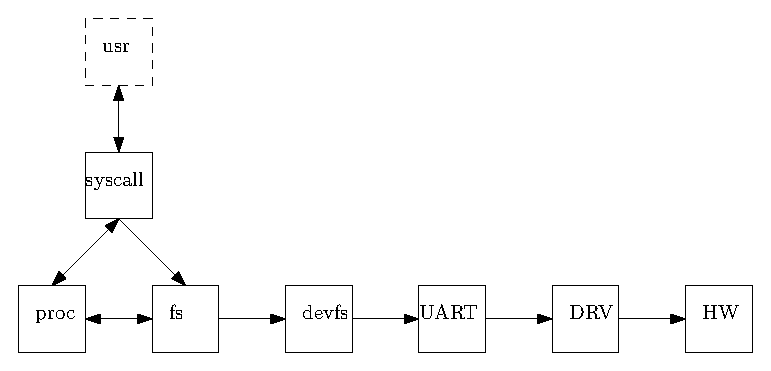
\includegraphics[width=9cm]{pics/uart}
  \caption{Communication between subsystems when a user process is writing to a UART.}
  \label{figure:dir}
\end{figure}


